\section{A triangle released from rest}\label{sec:intro}

Place three small, perfectly concentrated masses at the corners of a right
triangle. Give the triangle sides of length 3, 4, and 5, and give the bodies
masses 3, 4, and 5, placing each body opposite the side with its own number.
Let go of all three at once. There is no initial push, no friction, and no
force except their mutual Newtonian gravity. What happens?

At first the bodies fall toward one another. Later they can exchange
partners, pass extremely close, or fling one another far away. A particularly
appealing possibility is that they eventually come back to their starting
positions, stop together, and repeat the same dance forever. This paper
asks whether that can happen for \emph{any} integer right triangle when
its masses and opposite sides are tied together in this way. The conjecture
is that it cannot. We have substantial partial results, but no proof of the
universal claim and no counterexample.

\subsection{From Meissel's question to computer experiments}

The starting point is a conversation, rather than a known published
conjecture. In his 1913 paper, Carl Burrau recalled speaking in 1893 with
the Kiel mathematician Ernst Meissel, who believed that the $3$--$4$--$5$
initial conditions would produce periodic motion. Burrau also wanted to
test variable-step numerical integration on a demanding example. His
original account credits Sigurd Kristensen with a substantial part of the
calculation~\cite{Burrau1913}. The attractive integers made the experiment
easy to describe; they did not make its motion easy to calculate.

The decisive revival preceded the famous 1967 publications. Szebehely's
own account records calculations in 1966 by Standish at Yale, Spinelli
with Lecar and Szebehely at NASA's Institute for Space Studies, and Stanek
under Stiefel at ETH Z\"urich. It says that Szebehely suggested the revival,
but does not say how he first encountered Burrau's paper. We have found no
primary-source statement identifying a person or occasion that brought it
to his attention~\cite{Szebehely1967}.

Nor should the intervening years be described as a complete halt in work
on three bodies of comparable masses. Szebehely discusses Str\"omgren's
periodic-orbit work, Zumkley's 1941 integration, and Garcia's 1966 extension
of Zumkley's example~\cite{Szebehely1967}. Zumkley explicitly cites Burrau on the first page of his paper, but
uses three unit masses and a slide rule~\cite{Zumkley1941}. Str\"omgren's
1919 paper likewise studies a different periodic-orbit construction~\cite{Stromgren1919}.
These are related problems, not evidence that the exact $3$--$4$--$5$ trajectory was continuously
recomputed. The sources examined here do not establish a continuation of
that exact calculation between Burrau's work and the documented 1966
revival. This distinction is more defensible than a claim of fifty-four
years of complete silence.

Szebehely and C.~Frederick Peters followed the original motion far enough
to identify its eventual behavior: the two heavier bodies, of masses 4
and 5, form a binary, while the mass-3 body escapes. Their paper explains
that Burrau had stopped at $t=3.35$, before this outcome was apparent.
Their numerical resolution refuted Meissel's expectation for that particular
triangle~\cite{SP1967}. It did not settle every integer right triangle.
In a separate paper that year, they found a nearby periodic solution with
a binary collision and perturbed initial distances~\cite{SPPeriodic}.
That example is outside the collision-free question considered here.

\subsection{The modern question is more specific than free fall}

Starting from rest does not itself rule out periodic motion. Standish's
collisionless periodic example appeared in 1970~\cite{Standish1970}.
Kiyotaka Tanikawa, Hiroaki Umehara, and Hiroshi Abe developed systematic
searches for binary- and triple-collision orbits in 1995; Tanikawa's 2000
continuation studied the structure of this free-fall initial-condition
space~\cite{TUA,Tanikawa2000}. Their work makes collisions part of the
organization of the problem, rather than merely numerical inconveniences.
Moeckel, Montgomery, and Venturelli subsequently developed the rigorous
passage from a configuration at rest to the first collinear configuration,
and constructed periodic collision orbits in the isosceles
problem~\cite{MMV}. Montgomery's \emph{Dropping Bodies} gives a modern
account of periodic free-fall motion and its reversal symmetry~\cite{Montgomery}.
None of these statements identifies the all-integer nonperiodicity claim
of this paper as a conjecture due to Tanikawa or Montgomery.

Recent computations make the distinction still more important. Li and
Liao's 2019 catalogue reports 316 periodic free-fall solutions, including
313 new examples, for several mass ratios~\cite{LiLiao}.
Hristov, Hristova, Dmitra\v sinovi\'c, and Tanikawa's 2024 equal-mass search
reports 12,409 distinct solutions below its specified scale-invariant
period cutoff~\cite{Hristov}. These catalogues vary initial shapes more
freely than our experiment. Equal masses cannot satisfy our right-triangle
mass--side rule. Unequal-mass entries are useful starting guesses, but must
still satisfy both the mass--side relation and the right-angle equation.

The original Pythagorean problem also remains a numerical benchmark:
Rantala, Pihajoki, Mannerkoski, Johansson, and Naab use it to test their
2020 regularized integrator~\cite{Rantala}. Chitan, Myll\"ari, and Haque
revisited Pythagorean black-hole triples in 2022, and Chitan, Myll\"ari,
and Valtonen studied spin effects in 2025~\cite{Chitan2022,Chitan2025}.
Those relativistic extensions address encounters, escape, and mergers under
modified equations. They demonstrate continued interest in the experiment,
while leaving the exact Newtonian conjecture here open.

\subsection{One number specifies the experiment}

The rule ``mass equals opposite side'' is understood in chosen mass and
length units, with gravitational constant set to one. Enlarging all three
masses and all three lengths by the same factor changes the clock rate,
but preserves whether the motion repeats. We can therefore divide by the
hypotenuse and work with a longest side and largest mass equal to one.
Write the two other side lengths, and their corresponding masses, as
$A$ and $B$. The right-angle condition becomes $A^2+B^2=1$.

A convenient way to describe every such triangle is to slide a single
parameter $u$ through the interval $(0,1)$:
\begin{equation}\label{eq:parameter}
 A=\frac{1-u^2}{1+u^2},\qquad B=\frac{2u}{1+u^2}.
\end{equation}
Geometrically, if $(A,B)=(\cos\theta,\sin\theta)$, then
$u=\tan(\theta/2)$. No trigonometry is required to use the rational
formulas. If $u=p/q$ is a fraction in lowest terms, multiplying through
by $q^2+p^2$ gives Euclid's integer triple
\[
 (q^2-p^2,\ 2pq,\ q^2+p^2).
\]
Divide the triple by two when both $p$ and $q$ are odd. Conversely, every
primitive integer right triangle arises this way, allowing exchange of its
two legs. ``Primitive'' means that the three integers have no common
factor. For example, $u=1/2$ gives $(3,4,5)$, and $u=1/3$ gives $(4,3,5)$
after reduction. These are the same experiment with the first two labels
exchanged.

To avoid counting it twice, we use
\[
 0<u\le u_{\rm iso}:=\sqrt2-1,\qquad A\ge B.
\]
Near zero the triangle is very thin; at the other endpoint its two legs are
equal. That equal-leg endpoint has irrational $u$, so it belongs to the
continuous family used in the proof, but not to the integer conjecture.
Changing $u$ changes the masses \emph{and} the shape together. It does not
mean moving one body while keeping three arbitrary masses fixed.

\begin{figure}[tb]
\centering
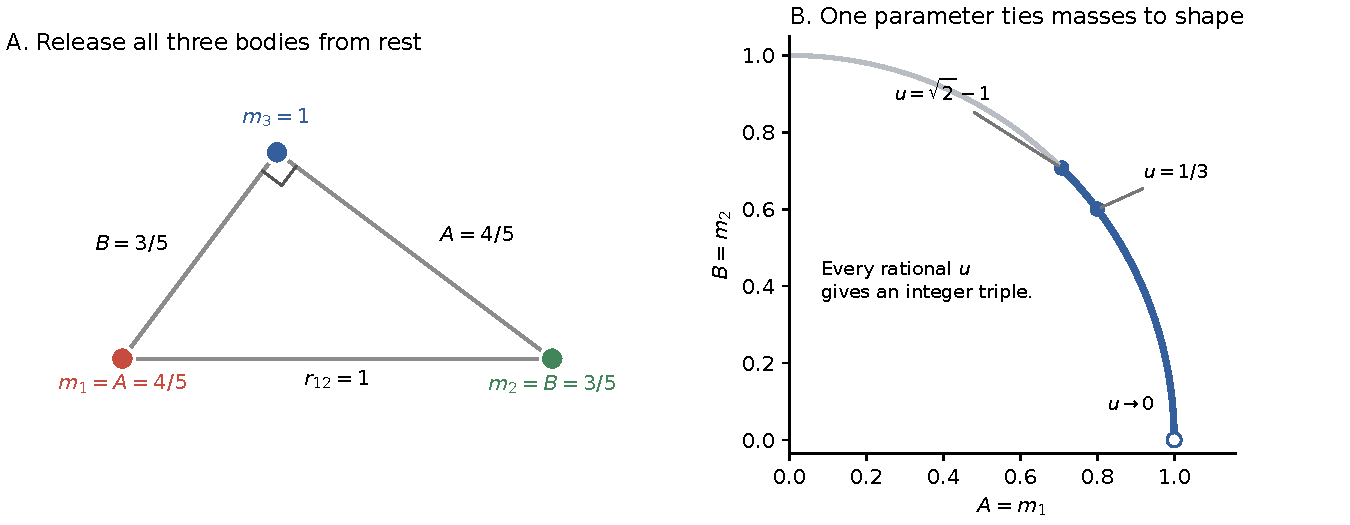
\includegraphics[width=\linewidth]{figures/initial-geometry.pdf}
\caption{The experiment and its parameter. Left: the normalized
$u=1/3$ triangle, with masses $(4/5,3/5,1)$ opposite equal-numbered side
lengths; all velocities initially vanish. Right: the allowed mass pairs
lie on the quarter unit circle. The darker arc is the fundamental interval
$0<u\le\sqrt2-1$; the thin-triangle endpoint $u=0$ is excluded. Rational
$u$, rather than arbitrary points selected numerically on the arc, produces
the integer triples.}
\label{fig:geometry}
\end{figure}

\subsection{What would count as a counterexample?}

A repeating picture is not enough. Each labelled body must return to its
own position with its own velocity in the same fixed coordinate frame,
without any collision along the way. A return after rotating the picture,
swapping bodies, or mathematically continuing through a collision does not
meet this definition. A numerical near-return, however precise, is a
candidate to investigate rather than an exact periodic orbit.

There is a useful simplification. Newton's equations work equally well
backward in time. If a collision-free trajectory that starts at rest ever
stops \emph{all three bodies simultaneously} a second time, it must retrace
its entire path and return to the beginning. Conversely, every periodic
trajectory starting at rest has such a second stop. Mathematicians call a
simultaneous stop a \emph{brake}. The conjecture can therefore be phrased
as: \emph{no integer Pythagorean experiment has a second brake before its
first collision}. Section~\ref{sec:search} describes our direct attempts
to find one.

\subsection{What the proof attempt achieves}

The difficulty is to control every future encounter for infinitely many
triangles. Figure~\ref{fig:fan} shows how nearby rational parameters can
produce visibly similar motion over a finite time, while close approaches
make numerical errors and small changes of parameter matter. A dense plot
is not a proof that a whole interval has been covered.

Three kinds of progress are established by the arguments and certificates
assembled here. First, an exact reduction identifies the only moments at
which a second brake is possible: strict maxima of the system's moment of
inertia, a measure of its overall spread. At such a maximum the changing
triangle still has to stop changing shape. Second, validated integration
and a forward escape estimate exclude every second brake on the explicit
real interval $[0.29,0.2900000101]$. Third, endpoint arguments give a
punctured neighborhood of the equal-leg triangle and infinitely many open
intervals accumulating at the thin-triangle end. On the explicit family
$(4n^2-1,4n,4n^2+1)$, the latter arguments cover a set of indices of positive
lower density: a positive fraction in the limiting lower-density sense,
not necessarily every large index.

These results leave much of the parameter interval unclassified. The
near-equal-leg cutoff is existential, and the thin-triangle result covers
escape windows rather than all phases. We also develop torque-history
identities that could help control the remaining region. The scalar
sign-change shortcut proposed in an earlier draft needs an additional
endpoint bound; Section~\ref{sec:torque} explains the correction. The
paper's outcome is a set of rigorous reductions and partial exclusions,
with the remaining global obligation stated explicitly.

\begin{figure}[p]
\centering
\begin{minipage}[c][.75\textheight][s]{.24\linewidth}
\raggedleft\small
\vspace*{.045\textheight}
$\Delta u=10^{-2}$\par\vfill
$\Delta u=10^{-2.5}$\par\vfill
$\Delta u=10^{-3}$\par\vfill
$\Delta u=10^{-3.5}$\par\vfill
$\Delta u=10^{-4}$\par
\vspace*{.065\textheight}
\end{minipage}\hspace{1em}%
\raisebox{-.5\height}{
\includegraphics[height=.75\textheight]{figures/oklo_pythagorean_fan_trajectory_progression.png}}
\caption{Progressively narrower collections of integer experiments near
$u=0.29$, using the project's original fan--trajectory visualization.
From top to bottom the intervals are $[0.29,0.29+\Delta u]$, with
$\Delta u=10^{-2},10^{-2.5},10^{-3},10^{-3.5},10^{-4}$.
Each left panel displays 400 primitive triples of smallest hypotenuse in
its interval, with radius on a common affine $\log_{10}c$ scale and its
angular interval expanded to one display radian. The highlighted sector
is the next narrower interval; large rings select ten triples whose
trajectories appear at right. Red, green, and blue track the three bodies
in the source plot's leg ordering. Right panels share one spatial scale,
show normalized physical times $0\le t\le4$, and clip outgoing paths.
Opacity decreases with body speed; it is not an integration-error measure.
Even the narrowest displayed interval is about 9,901 times wider than the
certified interval. This ordinary numerical illustration conveys the
search geometry, not validated parameter coverage.}
\label{fig:fan}
\end{figure}
